\documentclass[aspectratio=169]{beamer}
\usetheme{default}

\usepackage{amsmath,amssymb,mathtools}
\usepackage{tikz}

\title{A Bialgebra Framework for Positivity in Schubert Calculus}
\author{Matthew J. Samuel}
\institute{CombinaTexas 2026}
\date{2026}

\newcommand{\coma}{\mathcal{A}}
\newcommand{\dcoma}{\mathcal{D}}
\newcommand{\wb}[1]{\left[#1\right]}
\newcommand{\Sch}[1]{\Xi_{#1}}
\newcommand{\sch}{\mathfrak{S}}
\newcommand{\Key}[1]{\kappa_{#1}}
\newcommand{\Forest}[1]{\mathfrak{P}_{#1}}
\newcommand{\RC}{\mathrm{Pipe}}
\newcommand{\crossTile}{%
  \tikz[baseline=-0.6ex,scale=0.22]{%
    \draw[line width=0.45pt] (0,0) rectangle (1,1);
    \draw[line width=0.9pt] (0.12,0.5) -- (0.88,0.5);
    \draw[line width=0.9pt] (0.5,0.12) -- (0.5,0.88);
  }%
}
\newcommand{\bumpTile}{%
  \tikz[baseline=-0.6ex,scale=0.22]{%
    \draw[line width=0.45pt] (0,0) rectangle (1,1);
    \draw[line width=0.9pt] (0.5,0) .. controls (0.5,0.3) and (0.7,0.5) .. (1,0.5);
    \draw[line width=0.9pt] (0,0.5) .. controls (0.3,0.5) and (0.5,0.7) .. (0.5,1);
  }%
}
\makeatletter
\AtEndDocument{%
  \immediate\write\@auxout{\string\citation{mattsamuelcombinatexas2026dummy}}%
  \immediate\write\@auxout{\string\bibdata{mattsamuelcombinatexas2026_dummy}}%
  \immediate\write\@auxout{\string\bibstyle{plain}}%
}
\makeatother
\begin{document}

\begin{frame}
  \titlepage
\end{frame}

\begin{frame}{Plan}
\begin{itemize}
  \item Section 1: the ambient bialgebra object.
  \item Dual algebra and basis indexing.
  \item Schubert, key, and forest bases in one transition framework.
  \item Final point: positivity questions through structure constants.
\end{itemize}
\end{frame}

\section{Section 1: ambient object}

\begin{frame}{Ambient graded object}
Define
\[
\coma = \bigoplus_{n\ge 0} \coma_n,
\qquad \coma_n = \mathbb{Q}[x_1,\dots,x_n].
\]

Multiplication in $\coma$ is componentwise:
\begin{itemize}
  \item if $f,g\in \coma_n$, then $f\cdot g$ is the usual product in $\mathbb{Q}[x_1,\dots,x_n]$;
  \item if $f\in \coma_m$, $g\in \coma_n$ with $m\neq n$, then $f\cdot g=0$.
\end{itemize}

So each graded piece is a familiar polynomial ring, and cross-component products are trivial. The coproduct is
\[\Delta(x_c) = \sum_{ab = c} x_a \otimes x_b\]
where $x_a$ is the monomial corresponding to the weak composition $a$.
\end{frame}

\begin{frame}{Stable polynomial bases in $\coma$}
Fix a polynomial basis family $\{B^{(n)}\}_{n\ge 0}$ with $B^{(n)}\subset \coma_n$.

Examples used here:
\begin{itemize}
  \item Schubert basis,
  \item key basis,
  \item forest basis,
  \item word/monomial-type basis.
\end{itemize}

Any such stable basis in $\coma$ determines a dual basis in $\dcoma$.
\end{frame}

\section{Dual algebra $\dcoma$}

\begin{frame}{Dual indexing and product}
The dual algebra $\dcoma$ has a basis indexed by weak compositions in one standard model:
\[
\{\wb{\alpha} : \alpha \text{ a weak composition}\}.
\]

Dual product is concatenation:
\[
\wb{\alpha}\cdot \wb{\beta} = \wb{\alpha\,\beta}.
\]

Hence $\dcoma$ is a free associative algebra (tensor algebra on the generators $\wb{k}$, $k\ge 0$). The coproduct is
\[\Delta(\wb{\gamma}) = \sum_{\alpha + \beta=\gamma} \wb{\alpha} \otimes \wb{\beta}.\]
\end{frame}

\begin{frame}{Crossing diagrams}

Think of a one-row strip of $n-1$ boxes.

\begin{itemize}
  \item Label the left edge by $1$.
  \item Label the bottom by a permutation of the numbers $2,3,\dots,n$ (left to right).
  \item In each box, place either a \emph{cross} $\crossTile$ or a \emph{bump} $\bumpTile$.
\end{itemize}

\begin{center}
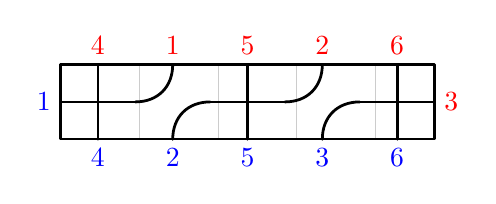
\begin{tikzpicture}[x=0.95cm,y=0.95cm,line cap=round,line join=round]
  % One-row grid paper
  \draw[gray!40, very thin] (0,0) grid (5,1);
  \draw[black, line width=0.8pt] (0,0) rectangle (5,1);

  % Cross tiles (plus shape, edge-center to edge-center)
  \foreach \c in {0,2,4}{
    \draw[line width=1.0pt] (\c,0.5) -- (\c+1,0.5);
    \draw[line width=1.0pt] (\c+0.5,0) -- (\c+0.5,1);
  }

  % Bump tiles (west->north and south->east)
  \foreach \c in {1,3}{
    \draw[line width=1.0pt] (\c+0.5,0) .. controls (\c+0.5,0.3) and (\c+0.7,0.5) .. (\c+1,0.5);
    \draw[line width=1.0pt] (\c,0.5) .. controls (\c+0.3,0.5) and (\c+0.5,0.7) .. (\c+0.5,1);
  }

  % Input labels (left and bottom)
  \node[left, text=blue] at (0,0.5) {$1$};
  \node[below, text=blue] at (0.5,0) {$4$};
  \node[below, text=blue] at (1.5,0) {$2$};
  \node[below, text=blue] at (2.5,0) {$5$};
  \node[below, text=blue] at (3.5,0) {$3$};
  \node[below, text=blue] at (4.5,0) {$6$};

  % Output labels after tracing strands (top, then right edge)
  \node[above, text=red] at (0.5,1) {$4$};
  \node[above, text=red] at (1.5,1) {$1$};
  \node[above, text=red] at (2.5,1) {$5$};
  \node[above, text=red] at (3.5,1) {$2$};
  \node[above, text=red] at (4.5,1) {$6$};
  \node[right, text=red] at (5,0.5) {$3$};
\end{tikzpicture}
\end{center}

Follow the strands through the row. The admissibility condition is that it cannot undo inversions, only create new ones.

\end{frame}

\begin{frame}{A nice combinatorial basis}
Let $\Xi_w^k$ be the basis indexed by permutations $w$ such that $w(p) < w(p+1)$ for all $p>k$ satisfying the following:
\begin{itemize}
\item $\Xi_{w}^1 = [w(1) - 1]$
\item For a nonnegative integer $[p]$, we have that
$$[p]\cdot\Xi_w^k = \sum_{w'}\Xi_{w'}^{k+1}$$
where $w'$ is obtained from $w$ through a valid crossing diagram with $p$ crosses after adding $1$ to each element of $w$ and adding a new first element $1$. 
\end{itemize}

I can provide an explicit (but mildly cancellative) formula for $\Xi_w^k$ in the word basis, as well as a positive formula for the product of $\Xi_u^p$ and $\Xi_v^q$ in terms of crossing diagrams. 

The coproduct structure constants are also nonnegative integers, but I do not have a positive combinatorial formula for them yet$\ldots$
\end{frame}

\begin{frame}{Taking off the mask: The dual Schubert basis}
The basis satisfies
$$\langle \mathfrak{S}_{u}(x_1,\ldots,x_n), \Xi_{v}^{n} \rangle = \delta_{u,v}$$
where $\mathfrak{S}_{u}(x_1,\ldots,x_n)$ is the Schubert polynomial corresponding to the permutation $u$.

\[
\Delta\,\Sch{w}^{n} = \sum_{u,v} c_{u,v}^{w}\,\Sch{u}^{n}\otimes \Sch{v}^{n}
\]

The coefficients $c_{u,v}^{w}$ are the Littlewood--Richardson type structure constants for the flag variety.

This is the main structural link: Schubert positivity data appears as bialgebra structure constants.

(Yes, the crossing diagrams are secretly pipe dreams.)
\end{frame}

% \begin{frame}{Theorem (placeholder): explicit LR rule in the dual Schubert basis}
% \textbf{Theorem.} \emph{(Placeholder for final statement.)}

% There is an explicit Littlewood--Richardson type rule for the concatenation product in the dual Schubert basis:
% \[
% \Sch{u}^{n_1}\cdot \Sch{v}^{n_2}
% =
% \sum_{w} c_{u,v}^{w}\,\Sch{w}^{n_1 + n_2},
% \]
% where $c_{u,v}^{w}$ are given by an explicit combinatorial counting rule.

% \vspace{0.5em}
% \textbf{To fill in during talk prep:}
% \begin{itemize}
%   \item precise combinatorial objects,
%   \item admissibility conditions,
%   \item exact indexing conventions.
% \end{itemize}
% \end{frame}

\begin{frame}{Bounded pipe dream ring product}
Bounded pipe dreams are pipe dreams together with an additional length parameter.

\vspace{0.4em}

\begin{itemize}
  \item There is an insertion-based reduction map from a pipe dream of length $n$ with empty row $n$ to a unique pipe dream of length $n-1$,
in a way that matches the Schubert transition formula in a strong, weight-preserving, bijective form.
\end{itemize}

Given bounded pipe dreams $R_1,R_2$, define $R_1\star R_2$ by:
\begin{itemize}
  \item \emph{untransitioning} $R_1$ in all possible valid ways to create space while remaining a pipe dream,
  \item shifting $R_2$ upward,
  \item placing the shifted $R_2$ into the new empty region, unchanged, if doing so yields a valid pipe dream.
\end{itemize}

This gives the product structure used in the pipe dream lift.
\end{frame}

\begin{frame}{Pipe dream ring as a lift of $\dcoma$}
There are two surjective linear maps from the pipe dream ring $\mathcal{R}$ to the dual algebra $\dcoma$:
\[
\pi_{\mathrm{Sch}}:\mathcal{R}\twoheadrightarrow \dcoma,\qquad
\pi_{\mathrm{Sch}}(G)=\Sch{\mathrm{perm}(G)}^{(n)},
\]
\[
\pi_{\mathrm{wt}}:\mathcal{R}\twoheadrightarrow \dcoma,\qquad
\pi_{\mathrm{wt}}(G)=\wb{\mathrm{wt}(G)}.
\]
By virtue of the fact that $\dcoma$ is free, there is a section $\iota:\dcoma\hookrightarrow \mathcal{R}$ of $\pi_{\mathrm{wt}}$ that sends $\wb{i}$ for an integer $i$ to the unique pipe dream $r_i$ with $\mathrm{wt}(r_i)=(i)$. It turns out that these are all ring homomorphisms and $\iota$ is also a section of $\pi_{\mathrm{Sch}}$.
\begin{theorem}
We have that $\pi_{\mathrm{Sch}}$ and $\pi_{\mathrm{wt}}$ are surjective ring homomorphisms to $\dcoma$ and $\iota$ is an injective ring homomorphism from $\dcoma$ to $\mathcal{R}$ such that
$$\pi_{\mathrm{Sch}} \circ \iota = \pi_{\mathrm{wt}} \circ \iota = \mathrm{id}_{\dcoma}.$$
\end{theorem}

% Hence pipe dreams are a bijective dictionary between the Schubert basis and the word basis that respects the algebra structure.
%Under the basis identification in $\dcoma$, these describe the same surjective ring homomorphism (Schubert coordinates versus word coordinates).
\end{frame}

\begin{frame}{Direct sum decomposition of $\mathcal{R}$}
Consider the two-sided ideal $I$ of $\mathcal{R}$ generated by $R_1 - R_2$, where $w(R_1) = w(R_2)$. Then $\mathcal{R} = I \oplus \iota(\dcoma)$ as a vector space, and the projection map $\pi_{\mathrm{Sch}}$ is the projection onto the second factor. In particular, $\iota(\dcoma)$ is a subalgebra of $\mathcal{R}$ isomorphic to $\dcoma$.

\begin{theorem}
If $\{\mathfrak{A}_\alpha\}$ is a Schubert positive homogeneous basis of $\dcoma$, then there is a unique representation
$$\iota(\mathfrak{A}_\alpha) = \sum_{w\in P_\alpha,R'\in \RC(w)}a_{\alpha}^{R'}R' + \sum_{R\in\RC\setminus I_\alpha} c_\alpha^R R$$
where $c_\alpha^R \geq 0$ for all $R$. 
% In this situation, choose $w$ such that $c_\alpha^R=1$ for some $R\in \RC(w)$. Then the dual basis $\{\mathcal{A}_\alpha\}$ in $\coma$ satisfies
% $$\mathcal{A}_\alpha = \sum_{R'\in\RC(w(R))} x_{\mathrm{wt}(R')}.$$
\end{theorem}
% Hence pipe dreams are a bijective dictionary between the Schubert basis and the word basis that respects the algebra structure.
%Under the basis identification in $\dcoma$, these describe the same surjective ring homomorphism (Schubert coordinates versus word coordinates).
\end{frame}

\begin{frame}{Immediate consequence}
We immediately obtain a formula for the product of dual Schubert elements.

\begin{theorem}
For dual Schubert elements $\Sch{u}^{n_1}$, $\Sch{v}^{n_2}$, we have
\[
\Sch{u}^{n_1}\cdot \Sch{v}^{n_2}
=
\sum_{w} d_{u,v}^{w}(n_1, n_2)\,\Sch{w}^{n_1 + n_2},
\]
where, fixing pipe dreams $R_u$ for $u$ and $R_v$ for $v$, $d_{u,v}^{w}(n_1, n_2)$ is the number of bounded pipe dreams $R_w\in\RC(w)$ such that $R_w$ has a coefficient of $1$ in the product $R_u\star R_v$.

Equivalently,
$$\sch_w(x_1,\ldots,x_{n_1+n_2}) = \sum_{u,v} d_{u,v}^{w}(n_1, n_2)\,\sch_u(x_1,\ldots,x_{n_1})\sch_v(x_{n_1+1},\ldots,x_{n_1+n_2}).$$
\end{theorem}

\end{frame}


\begin{frame}{Positivity theorem}
\begin{theorem}
Suppose there is an equivalence relation on reduced words $\equiv$ such that the following hold:

If $W,W'$ are reduced words such that $W\equiv W'$, then
\begin{itemize}
\item ${\uparrow}W\equiv {\uparrow}W'$.
\item $\mathrm{perm}(W) = \mathrm{perm}(W')$.
\item If $i$ is the last descent of $\mathrm{perm}(W)$, then $L_{i,i+1}(W)\equiv L_{i,i+1}(W')$.
\end{itemize}
Then there is a unique family of polynomials with nonnegative integer coefficients $\{\mathfrak{A}_\alpha\}$ that form a basis for $\coma$ such that $\mathfrak{A}_\alpha$ is the sum of monomials corresponding to pipe dreams with reduced words in the equivalence class $P_\alpha$ of $\equiv$. The dual basis $\{\mathcal{A}_\alpha\}$ in $\dcoma$ is then positive in the dual Schubert basis and has nonnegative structure constants.
\end{theorem}
\end{frame}

\begin{frame}{Examples}

\begin{theorem}
  \begin{itemize}
  \item Schubert polynomials: $\mathrm{perm}(W) = \mathrm{perm}(W')$.
  \item Fundamental slide polynomials
  \item Key polynomials: $W\equiv W'$ if $W$ and $W'$ are Coxeter-Knuth equivalent.
  \end{itemize}
% For dual key elements $\kappa_\alpha$, $\kappa_\beta$, we have
% \[
% \kappa_\alpha \cdot \kappa_\beta
% =
% \sum_{\gamma} d_{\alpha,\beta}^{\gamma}\,\kappa_\gamma,
% \]
% where, fixing a highest weight pipe dream $R_\gamma$ with $\alpha(R_\gamma)=\gamma$, $d_{\alpha,\beta}^{\gamma}$ is the number of pairs of highest weight
% bounded pipe dreams $R_\alpha, R_\beta$ with $\alpha(R_\alpha)=\alpha$ and $\alpha(R_\beta) = \beta$ such that $R_\gamma$ has a coefficient of $1$ in the product $R_\alpha\star R_\beta$.
\end{theorem}

\end{frame}

\begin{frame}{Forest polynomials}
Forest polynomials $\Forest{F}$ are a more recently discovered basis of $\coma$ in which the Schubert basis also expands positively. The
forest expansion of a Schubert polynomial is given by counting equivalence classes of reduced words for a permutation. We give a new result:

\begin{theorem}
Let $\mathcal{C}$ be an $\Omega$-invariant of a pipe dream, say for a permutation $w$, such that $\mathrm{shape}(\mathcal{C}) = F$. Then
$$\Forest{F}= \sum_{\substack{R\in\RC(w)\\\Omega(R) = \mathcal{C}}} \mathrm{wt}(R)$$
\end{theorem}


\end{frame}

\begin{frame}{Dual product of forest polynomials}
\begin{theorem}
  For dual forest elements $\Forest{F}$, $\Forest{G}$, we have
\[
\Forest{F} \cdot \Forest{G}
=
\sum_{\gamma} d_{F,G}^{H}\,\Forest{H}
\]

Where, fixing a pipe dream $R_H$ with $\Omega(R_H)$ has shape $H$, $d_{F,G}^{H}$ is the number of pairs of pipe dreams $R_F, R_G$ with 
$\mathrm{shape}(\Omega(R_F)) = F$ and $\mathrm{shape}(\Omega(R_G)) = G$ such that $R_H$ has a coefficient of $1$ in the product $R_F\star R_G$.

lebeled lbs
\end{theorem}
\end{frame}
% \section{Key and forest endpoint}

% \begin{frame}{Key and forest bases inside one framework}
% Inside $\coma_n$, one has expansions such as
% \[
% \Sch{w}(x) = \sum_{\alpha} a_{w,\alpha}\,\Key{\alpha}(x),
% \qquad
% \Sch{w}(x) = \sum_{\beta} b_{w,\beta}\,\Forest{\beta}(x),
% \]
% with nonnegative coefficients in many cases of interest.

% Dual bases in $\dcoma$ reflect these same transition coefficients.
% \end{frame}


% \begin{frame}{Forest culmination}
% For this talk, the endpoint is the forest basis:
% \begin{itemize}
%   \item Schubert-to-forest positivity in $\coma$,
%   \item corresponding dual basis transitions in $\dcoma$,
%   \item combinatorial interpretations suggested by the same bialgebra structure.
% \end{itemize}

% This places recent forest polynomial results in the same algebraic framework as earlier Schubert/key positivity.
% \end{frame}

% \begin{frame}{Summary}
% \begin{itemize}
%   \item $\coma=\bigoplus_n \mathbb{Q}[x_1,\dots,x_n]$ with componentwise multiplication.
%   \item Stable polynomial bases in $\coma$ give dual bases in $\dcoma$.
%   \item $\dcoma$ is free under concatenation product.
%   \item Schubert coproduct in $\dcoma$ carries LR-type flag-variety constants.
%   \item Forest positivity is a natural final example in this framework.
% \end{itemize}
% \vspace{0.4em}
% \centering
% Thank you.
% \end{frame}

\end{document}
